\documentclass{beamer}
\usetheme{CambridgeUS}
%Information to be included in the title page:
\institute{UNIVERSITATEA ”ALEXANDRU-IOAN CUZA” DIN IAȘI}
\title{Music Recognition Using Convolutional Neural Networks}
\\
\\
\author{{Absolvent: Vavilov Andrei} \\
{\and} \\
{Coordonator științific: Conf. Dr. Vitcu Anca} }
\date{Sesiunea: Iulie 2021}

\begin{document}

\frame{\titlepage}

\begin{frame}
\frametitle{Table of Contents}

\begin{itemize}
	\item Motivation
	\item Personal contributions
	\item Application architecture
	\item Demo
	\item Possible improvements
	\item Conclusion
	\item Bibliography
\end{itemize}
\end{frame}

\begin{frame}
\frametitle{Motivation}
\begin{itemize}
	\item The need for a application which combines neural networks with
	the arts domain.
	\item The need for an interactive way to visualise an application based
		on convolutional neural networks.
	\item A mean to integrate 3D Models into user friendly applications.
\end{itemize}


\end{frame}

\begin{frame}
\frametitle{Personal contributions}
\begin{itemize}
	\item The implementation approach of the neural network framework
	\item Simplifying the user interaction with the trained model based on the aforemetioned framework.
	\item Providing of a simplistic interface to visualize and classify a song based on its YouTube link
	\item Making the application more user friendly by incorporating two 3D animations in order to enhance the visual experience.
\end{itemize}`
\end{frame}

\begin{frame}
\frametitle{Application architecture}
The application is divided into three parts:
\begin{itemize}
	\item The Neuronal Network Engine
	\item The User Input Handling and Processing
	\item The Application-User interaction via the GUI
\end{itemize}
The application architecture is illustrated in the below figure:
\begin{center}
	\centering
	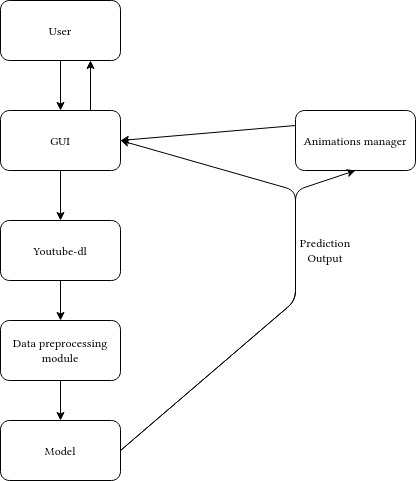
\includegraphics[width = 1.5in]{images/fac.png}
	\centerline{\captionof{Figure: Application architecture}}
	\label{uc1}
	\end{center}
\end{frame}
\begin{frame}
\frametitle{Demo}
\end{frame}

\begin{frame}
\frametitle{Possible improvements}

\begin{itemize}
	\item Implementing more classes in order to represent multiple instruments.
	\item Designing and adding more 3D animations.
	\item Implemetinging GPU support for numeric operations.
\end{itemize}
\end{frame}

\begin{frame}
\frametitle{Conclusions}
\begin{itemize}
	\item The application succeeds in creating a middle way between art and computer science.
	\item The application provides a complex and comprehensive artificial intelligence background.
	\item The application corresponds with the initial ambitions of the project.
\end{itemize}
\end{frame}

\begin{frame}
\frametitle{Bibliography}
\begin{itemize}
	\item Harrison Kinsley and Daniel Kukieła. Neural Networks from Scratch in Python.
2020.
	\item Seth Adams. “Audio Classification”. In: (2020).

	\item Erik Lindernoren. “Machine Learning From Scratch”. In: (2019).

\end{itemize}
\end{frame}
\end{document}
